\documentclass[a4paper,twoside,11pt]{article}
\usepackage{a4wide,graphicx,fancyhdr,amsmath,amssymb,algpseudocode,algorithm,enumerate,hyperref,float,caption,subcaption}
\usepackage[english]{babel}
\numberwithin{equation}{section}

%----------------------- Macros and Definitions --------------------------

\setlength\headheight{20pt}
\addtolength\topmargin{-10pt}
\addtolength\footskip{20pt}

\newcommand{\N}{\mathbb{N}}
\newcommand{\ch}{\mathcal{CH}}

\fancypagestyle{plain}{%
\fancyhf{}
\fancyhead[LO,RE]{\sffamily\bfseries\large}
\fancyhead[RO,LE]{\sffamily\bfseries\large }
\fancyfoot[LO,RE]{\sffamily\bfseries\large }
\fancyfoot[RO,LE]{\sffamily\bfseries\thepage}
\renewcommand{\headrulewidth}{0pt}
\renewcommand{\footrulewidth}{0pt}
}

\pagestyle{fancy}
\fancyhf{}
\fancyhead[RO,LE]{\sffamily\bfseries\large Project 2ID35}
\fancyhead[LO,RE]{\sffamily\bfseries\large Eindhoven University of Technology}
\fancyfoot[LO,RE]{\sffamily\bfseries\large }
\fancyfoot[RO,LE]{\sffamily\bfseries\thepage}
\renewcommand{\headrulewidth}{1pt}
\renewcommand{\footrulewidth}{0pt}

%-------------------------------- Title ----------------------------------

\title{\vspace{-\baselineskip}\sffamily\bfseries Deliverable 1 2ID35 \\ Database Technology }

\author{
C. Lambrechts - 0733885 - {\tt c.lambrechts@student.tue.nl} \\
K. Triantos - 0852612 - {\tt k.triantos@student.tue.nl}\\
J. Wulms - 0747580 - {\tt j.j.h.m.wulms@student.tue.nl}\\
}

\date{\today}

%--------------------------------- Text ----------------------------------

\begin{document}
\maketitle
\thispagestyle{empty}
\begin{abstract}
This report contains the first deliverable of the project for the course 2ID35 Database Technology. We provide some background for the paper we are studying, work out the research problems that have been addressed and what results have been claimed by the paper. We then proceed by giving an overview of what we are going to do in order to verify the research that has been done by the authors of the paper, and a discussion of the results so far.
\end{abstract}

\section{Introduction} \label{sec:Introduction}
Optimizing a query can be done in several ways. The operation that is the computational most expensive is the join operation. So it makes sense to try to make this operation faster. Changing the order in which joins are performed is a common approach. For this approach cost approximations are computed before actually performing the joins. This approach requires  the development of a cost model, an assignment of an estimated cost to each query processing plan and searching in the (huge) search space for the cheapest cost plan. There are also approaches that do not use cost plans. One of the approaches focusses on minimizing the number of joins instead of using a optimal join order. This approach requires a homomorphism test, which is NP-complete. An other approach focusses on the structural properties of the queries. It will try to find a project-join order that will minimize the size of the intermediate results during query evaluation. Practical it means, use only the data that you need and remove the rest as soon as possible. \\

The paper \cite{paper} we are reviewing develops such a structural approach. The authors of that paper try to push down the projections, such that the attributes that are not needed are projected out as early as possible. The projection pushing strategy has been applied to solve constraint satisfaction problems in Artificial Intelligence with good experimental results. The input to a constraint-satisfaction problem consists of a set of variables, a set of possible values for the variables, and a set of constraints between the variables; the question is to determine whether there is an assignment of values to the variables that satisfies the given constraints. IN the database area, this means that you are searching for entries that satisfy the constraints on their attributes. \\

Optimizing the query manually, often focusses on reducing the search space before the join operation. In this fashion the number of entries used in the join is less, which can result in a huge performance gain. Most of the time the projections are pushed down by selecting as soon as possible or pushing the projection to a sub query. It is possible to make a sub-query that projects out all irrelevant information and tries to reduce the intermediate results. Optimizing the query in an automated and structural way looks promising and practical.  \\

We start by presenting the problem description found in the paper in Section~\ref{sec:ProblemDescription}. Then the results claimed in the paper are discussed, Section~\ref{sec:ClaimedResults}. To verify the results we present our methodology in Section~\ref{sec:Methodology}. Section~\ref{sec:Discussion} discusses the current progress and the current state of the implementation.

\section{Problem Description} \label{sec:ProblemDescription}
\section{Problem Description}


\section{Claimed Results} \label{sec:ClaimedResults}
In order to verify the paper we are looking into, we need a precise overview of the results that are claimed by the authors of the paper. This way we are able to make clear comparisons between the claimed results and our own.

\subsection{Paper results}
We first look at the results for the 3-COLOUR graphs where order is fixed and the density scales:
\begin{enumerate}
	\item \label{claim:Curve} The curves for Boolean and non-Boolean queries have roughly the same shape.
	\item \label{claim:RunInc} At first the running time increases as density increases, because of an increased number of joins.
	\item \label{claim:SizeInter} Eventually the size of intermediate results becomes small or empty, and additional joins have little effect on overall running time.
	\item \label{claim:IncImprov} At low density each optimization method improves upon the previous. For denser instances, optimizations using early projection lose their effectiveness.
	\item \label{claim:BucketDominates} Bucket elimination completely dominates the greedy methods.
\end{enumerate}

\noindent Proceeding with the results for 3-COLOUR graphs where density is fixed and the order scales. The density is fixed at 2 values, and the authors assume that the lower value is most likely associated with 3-colourable graphs, and the higher density with non-3-colourable graphs:

\begin{enumerate}[resume]
	\item \label{claim:ExpoInc} All methods show exponential increase in running, when order is increased. (This is shown by a linear slope in log-scale.)
	\item \label{claim:BucketExpoImpr} Bucket elimination maintains a lower slope in log-scale, in comparison to the other optimizations. This lower slope in log-scale translates to a strictly smaller exponent, so we have an exponential improvement.
\end{enumerate}

\noindent The next focus of the report was order-scaling experiments with structured queries. We first look into augmented path instances:

\begin{enumerate}[resume]
	\item \label{claim:AugBucketDom} Bucket elimination is again the best, but early projection is competitive for these instances, because the problem has a natural order that works well for early projection.
	\item \label{claim:AugNonBool} For non-Boolean graphs the optimizations do not scale as well as for Boolean graphs. This is due to the fact that there are {\b 20\% less vertices to exploit in the optimization}. Early projection and bucket elimination still dominate the other optimizations in this case.
\end{enumerate}

\noindent The final claims are about the results for ladder graph instances, and augmented ladder instances:
\begin{enumerate}[resume]
	\item \label{claim:AugLadReordering} For ladder instances, the heuristic for reordering is not only unable to find a better order, but actually finds a worse one.
	\item \label{claim:AugLadSimilar} Furthermore, ladder instances give results very similar to augmented path instances.
	\item \label{claim:AugLadMoreDiff} Augmented ladder instances shows even more differences between optimization methods.
	\item \label{claim:AugLadNonBool} Non-Boolean cases for augmented ladder instances struggle to reach order 20 with the faster optimizations.
\end{enumerate}

\noindent The conclusion for all these results is that bucket elimination dominates the field at every turn with an exponential improvement. In a discussion about future research areas, the authors also claim that they found results consistent with 3-COLOUR queries, when using 3-SAT and 2-SAT to construct queries.

\subsection{Verification}
In our verification, the main claims we want to verify are the domination of bucket elimination and the exponential improvement it shows in the paper. The next step is going into the details of all the different query types (random and structured), and getting consistent results there, or finding out why we have different results. We will not look further look into queries constructed from other sources than 3-COLOUR, such as 3-SAT or 2-SAT.

\section{Methodology} \label{sec:Methodology}
\section{Methodology}
This section will elaborate on the steps we are going to take to verify the results in the paper.

\begin{figure}
	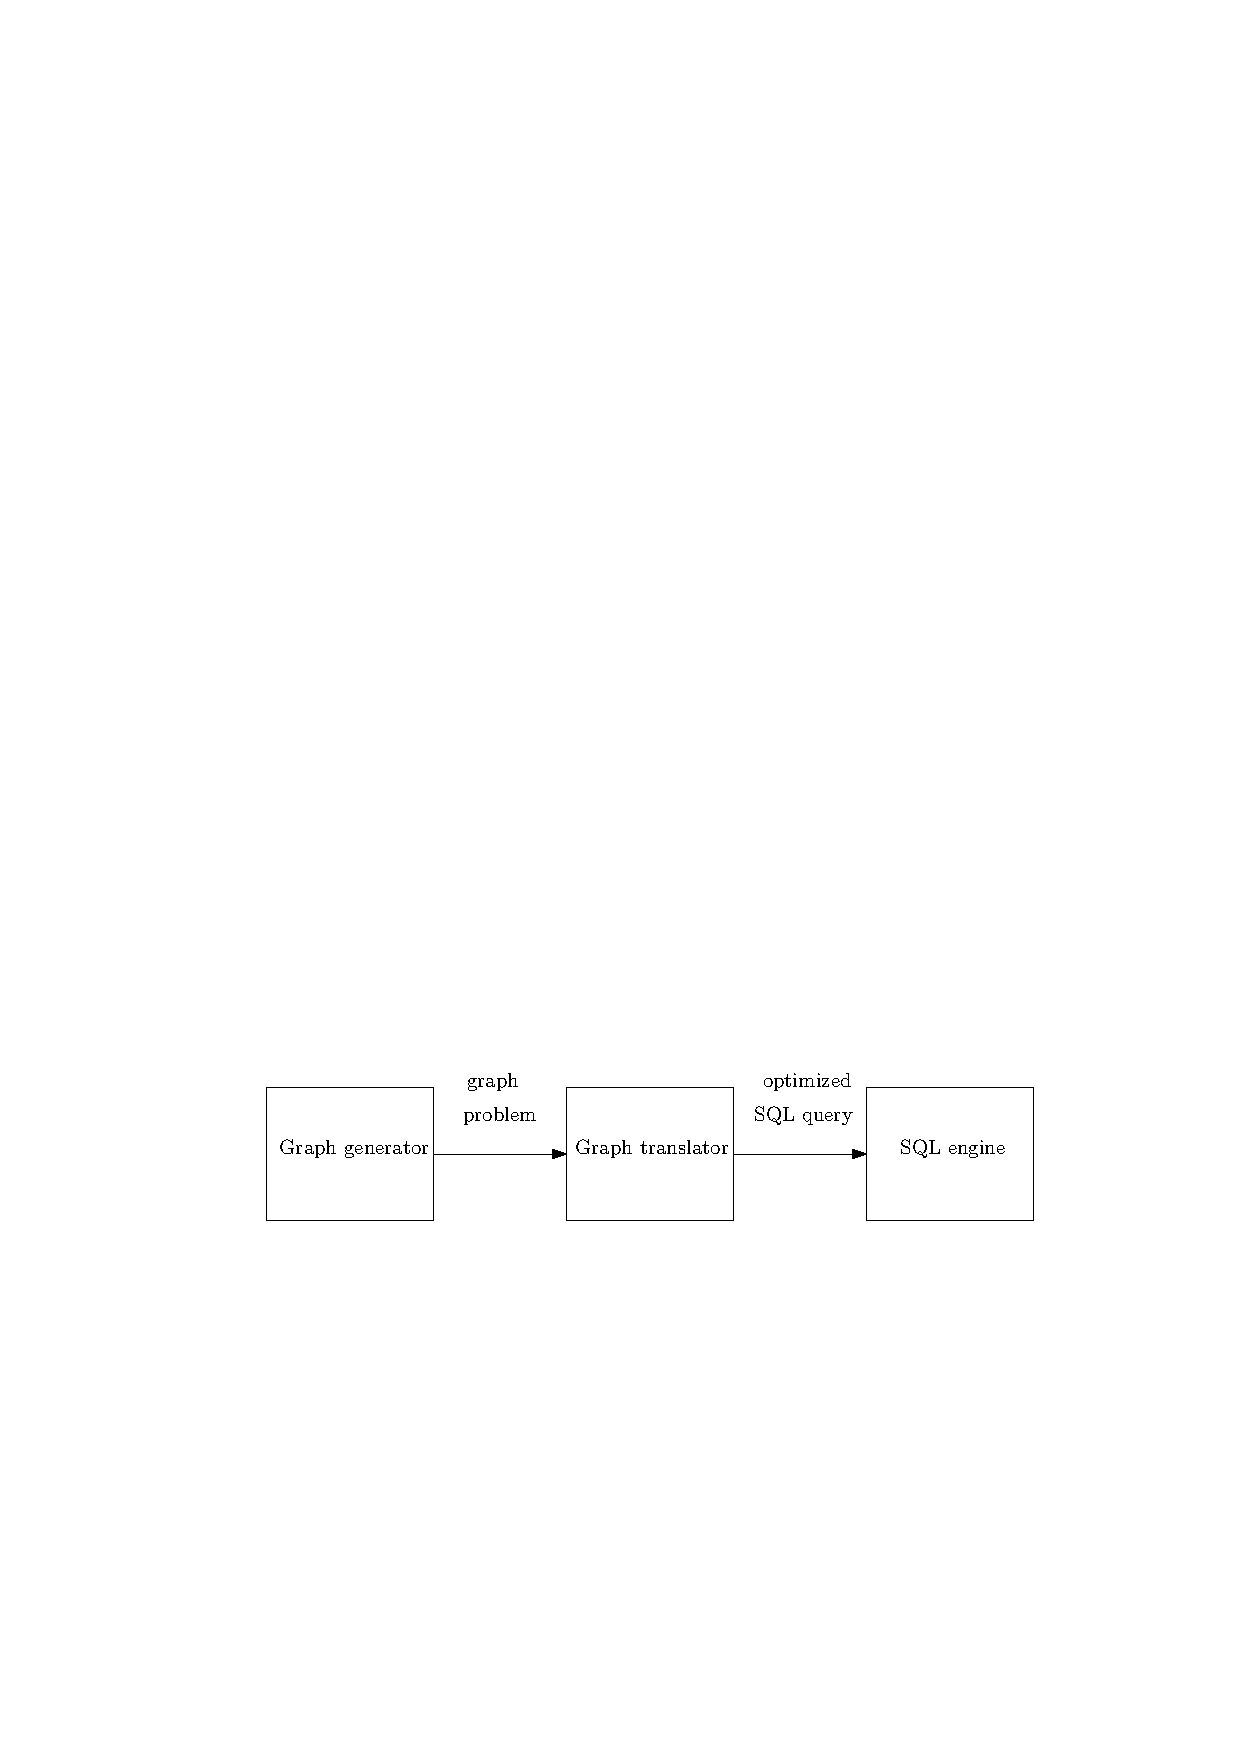
\includegraphics{figures/process.pdf}
	\caption{All steps in the process of verification}
	\label{fig:process}
\end{figure}

\section{Discussion of Progress} \label{sec:Discussion}
In this section we will discuss the results and try to verify the claims made by the authors of our paper \cite{paper}. We will start by discussing our findings and then we will compare them to the findings of our paper \cite{paper}.

\subsection{Our Findings} \label{subsec:DissFindings}
From the graphs presented in Section~\ref{sec:Results} (Figure~\ref{fig:ResultsRandomOrder}, Figure~\ref{fig:ResultsRandomDensity2} and Figure~\ref{fig:ResultsRandomDensity3}) we can see that all approaches are exponential in performance. There are differences between the approaches however. The naive approach is faster then the other approaches in the long run. It starts slower, but in the long run it becomes faster. We can see this by looking at the steepness of the trend line. This also hints us that the naive approach is faster for the fixed density of 0.6, but the steepness of the trend line is higher. So in the long run it will become slower. The other approaches seem similar in performance. Those trend lines are almost on top of each other. 

We think this has to do with the combination of the density and the order. A higher density means that it is less likely to be 3-colour able. With a low density the naive approach benefits from the fact that there are a lot of nodes not connected to each other. Unconnected nodes to not lay constraints on each other. This means that when a unconnected node is added, the Cartesian product needs to be computed. Due to the way the naive approach works, the Cartesian product is already created and only needs to be filtered on. This could also explain why the other approaches are slower. The other approaches uses joins, which are not optimal to compute Cartesian products. They are optimized for joining tables. Which is beneficial in the higher density setting. More connected nodes, means more joins. 

Besides these explanation, we think there could be another explanation for the differences. We generate the queries and send them to PostgreSQL, which executes them. It is almost certain that PostgreSQL tries to optimize the queries, before he actually executes them. The naive approach is quite clear and simple and therefore it is quit likely that the optimizer finds a way to make it faster. It is likely that the optimizer notices that he can rewrite the query, with some smart order of joining for example. For the straightforward approach this could be true, but it already uses joins. The order of the joins is already specified, which would make it harder for the optimizer to optimize. For the early projection and reordering approach it is unlikely that the optimizer finds a way to optimize it. Those queries are complicated and are already fixed by the query generator. 

\subsection{Comparison of the Findings} \label{subsec:DissComparison}
Before we start the comparison, lets filer out all comparison that are actually applicable to our experiments. The conclusion of the authors of our paper \cite{paper} was that bucket elimination dominates. We cannot check this conclusion due a unstable implementation, as mentioned before. This means that we can only verify or reject a claim for the random graph type and the naive, straightforward, early projection and reordering approach. The claims we can verify can be found below: 

\begin{enumerate}
\item[\ref{claim:RunInc}] At first the running time increases as density increases, because of an increased number of joins.
\item[\ref{claim:SizeInter}] Eventually the size of intermediate results becomes small or empty, and additional joins have little effect on overall running time.
\item[\ref{claim:IncImprov}] At low density each optimization method improves upon the previous. For denser instances, optimizations using early projection lose their effectiveness.
\item[\ref{claim:ExpoInc}] All methods show exponential increase in running, when order is increased. (This is shown by a linear slope in log-scale.)
\end{enumerate}

The general claims about the increase in performance when density increases (\ref{claim:RunInc} and the exponential increase in performance when order increases \ref{claim:ExpoInc} are verified. This can be seen in all graphs (Figure~\ref{fig:ResultsRandomOrder}, Figure~\ref{fig:ResultsRandomDensity2} and Figure~\ref{fig:ResultsRandomDensity3}) as all trend lines are increasing. 

The next claim we can verify, is the claim about the low density (\ref{claim:IncImprov}). We can say that we cannot verify this claim, as each optimization performs less than the naive approach. With the results we could even say that we reject the claim. As mentioned before this could be caused by the optimizer of PostgreSQL and by the number of joins that compute a Cartesian product.

The claim about the intermediate results (\ref{claim:SizeInter}) is harder to verify. We can implicitly verify it. We noticed that the queries that uses joins are performing worse than those that do not use joins (the naive approach). We know that joins are better at performing joins. There are two paths we can take to verify this claim. The first is by using the variables that are used in the join and the second is by using the intermediate sets. When the variables that are used for the join are not common, the Cartesian product is computed. If the intermediate results would be smaller or empty, this operation is more efficient. Hence the performance would be better. This is not the case as it performs worse than the naive approach, even in the long run. Now lets take the other path. If the intermediate results becomes smaller or empty, there less common variables to join on. Which would imply that there are more Cartesian products computed and thereby the performance becomes worse. Which can be seen in the results. Both the paths argue that this claim can be rejected.

%\nocite{*}
%\bibliographystyle{plain}
\bibliographystyle{is-abbrv}
\bibliography{ref}

\end{document}
